\documentclass[preprint,12pt]{elsarticle}

\usepackage{amssymb}

\usepackage{lineno}
\usepackage{hyperref}
\usepackage{quoting}
\usepackage{float}
\usepackage{lipsum}
\usepackage{tikz}
\usetikzlibrary{shapes,arrows,chains}
\usepackage{minted}
\usepackage{python}
\usepackage{amsmath}
\usetikzlibrary{matrix,shapes,arrows,positioning,chains}

\usepackage[autolinebreaks,useliterate]{mcode}

\begin{document}
	
	\tikzset{
		desicion/.style={
			diamond,
			draw,
			text width=3em,
			text badly centered,
			inner sep=0pt
		},
		block/.style={
			rectangle,
			draw,
			text width=18em,
			text centered,
			rounded corners
		},
		cloud/.style={
			draw,
			ellipse,
			minimum height=2em
		},
		descr/.style={
			fill=white,
			inner sep=2.5pt
		},
		connector/.style={
			-latex,
			font=\scriptsize
		},
		rectangle connector/.style={
			connector,
			to path={(\tikztostart) -- ++(#1,0pt) \tikztonodes |- (\tikztotarget) },
			pos=0.5
		},
		rectangle connector/.default=-2cm,
		straight connector/.style={
			connector,
			to path=--(\tikztotarget) \tikztonodes
		}
	}

\begin{frontmatter}

\title{Compressione di immagini tramite DCT\\
\large{Attraverso l'utilizzo di Python}
\vspace{5mm}\\ \normalsize{\texttt{https://github.com/nicoripa/MCS\_Project/}}}

\author{Lorenzo Rovida, Nicolò Ripamonti\\
	\small{ \href{mailto:l.rovida1@campus.unimib.it}{l.rovida1@campus.unimib.it},  \href{mailto:n.ripamonti@campus.unimib.it}{n.ripamonti@campus.unimib.it}\\817151, 816171}}

\address{Dipartimento di Informatica, Sistemi e Comunicazione, Universitá degli Studi di Milano-Bicocca, Milano, Italia}


\begin{abstract}
Lo scopo di questo progetto è quello di utilizzare l’implementazione dell'operazione matematica denominata \textbf{DCT2} in un ambiente \textit{open source} e di studiare gli effetti di un algoritmo di compressione di tipo jpeg (senza utilizzare una matrice di quantizzazione) sulle delle immagini in toni di grigio di formato \textit{bitmap}.
Il progetto si divide in tue macro parti:
\begin{description}
\item[Parte 1] Implementare la DCT2  in un ambiente open source a scelta e confrontare i tempi di esecuzione con la DCT2 ottenuta usando la libreria dell’ambiente utilizzato. In particolare, bisogna utilizzare array quadrati $N \times N$ con $N$ crescente e rappresentare su un grafico i tempi di esecuzione dei due algoritmi.
\item[Parte 2] Scrivere un software in grado di far scegliere all'utente un'immagine in formato bitmap e successivamente comprimere tale immagine utilizzando la DCT2, tagliare le frequenze che l'utente sceglie di eliminare, utilizzare l'inversa della DCT e far visualizzare a schermo l'immagine originale con quella ottenuta dopo aver modificato le frequenze.
\end{description}
\end{abstract}

\end{frontmatter}

\newpage

\section{Introduzione}
\subsection{Discrete Cosine Transform}
La trasformata discreta del coseno o DCT, è la più diffusa funzione che provvede alla compressione spaziale, capace di rilevare le variazioni di informazione tra un'area e quella contigua di un'immagine digitale trascurando le ripetizioni.

È una trasformata simile alla trasformata discreta di Fourier (DFT), ma fa uso solo di numeri reali.

La variante più comune della trasformata discreta del coseno è la DCT tipo II che è spesso chiamata semplicemente DCT; la sua inversa, la DCT tipo III è, in corrispondenza, chiamata spesso DCT inversa o IDCT. 

La DCT, e in particolare la DCT-II, è spesso usata nell'elaborazione dei segnali e delle immagini, specialmente per la compressione con perdita (compressione di tipo \textbf{lossy}). L'algoritmo JPEG è basato sulla Trasformata discreta del coseno bidimensionale (DCT2), che viene applicata su blocchi di 8x8 pixel, i cui risultati sono poi quantizzati e compressi con tecniche basate sull'entropia (come la Codifica di Huffman o la Codifica aritmetica).

\bigskip
La formula che descrive il funzionamento della DCT bidimensionale è la seguente:
\begin{eqnarray*}
c_{kl} = a_{kl} \sum_{i=0}^{N-1} \sum_{j=0}^{M-1} f_{ij} \,  cos\left(k\pi \frac{2i+1}{2N}\right) \, cos\left(l\pi \frac{2j+1}{2M}\right)
\end{eqnarray*}

Dove $a_{kl} = a_{k}^{N} a_{l}^{M}$:
\begin{eqnarray*}
a_{00} = \frac{1}{\sqrt{NM}},\; e \; a_{k0} = a_{0l} = \sqrt{\frac{2}{NM}},\; a_{kl} = \frac{2}{\sqrt{NM}}, \; k, l \geq 1.
\end{eqnarray*}

Mentre $f_{ij}$ sono gli indici bidimensionali:
\begin{eqnarray*}
\textbf{f} = (f_{ij}), \; i=0, ..., N-1, j=0, ..., M-1.
\end{eqnarray*}

\subsection{.Formato bitmap}
Windows bitmap è un formato dati utilizzato per la rappresentazione di immagini \textbf{raster} sui sistemi operativi Microsoft Windows. Noto soprattutto come formato di file, fu introdotto con Windows 3.0 nel 1990.
Le bitmap, come sono comunemente chiamati i file d'immagine di questo tipo, hanno generalmente l'estensione \textbf{.bmp}.

Sono state sviluppate tre versioni del formato bitmap. La prima e più comunemente utilizzata è la versione 3: non esistono versioni antecedenti. Le versioni successive 4 e 5 si incontrano piuttosto raramente.

Il formato di file Windows bitmap nella versione 3 permette operazioni di lettura e scrittura molto veloci e senza perdita di qualità, ma richiede generalmente una maggior quantità di memoria rispetto ad altri formati analoghi.

Le immagini bitmap possono avere una profondità di 1, 4, 8, 16, 24 o 32 bit per pixel. Le bitmap con 1, 4 e 8 bit contengono una tavolozza per la conversione dei (rispettivamente 2, 16 e 256) possibili indici numerici nei rispettivi colori. Nelle immagini con profondità più alta il colore non è indicizzato bensì codificato direttamente nelle sue componenti cromatiche RGB; con 16 o 32 bit per pixel alcuni bit possono rimanere inutilizzati.

Nel caso in esame le immagini in formato \textit{.bmp} sono state scelte con colori in scala di grigi, ovvero immagini con una profondità di 8 bit. Tali bit servono per convertire gli indici numerici nei rispettivi bit, in questo caso da 0, che identifica il colore nero, a 255, che identifica il colore bianco. Tutti i valori tra l'1 e il 254 sono tutte le possibili varianti di grigio.

\subsection{Calcolatore utilizzato}
Per effettuare i calcoli sugli script è stato utilizzato un MacBook Pro 2016 con le seguenti caratteristiche hardware:
\begin{description}
\item[Processore] 2 GHz Intel Core i5 dual-core
\item[Architettura] CPU x64
\item[Memoria] 8 GB 1867 MHz LPDDR3
\item[Scheda grafica] Intel Iris Graphics 540 1536 MB
\end{description}

\newpage

\section{Ambiente di sviluppo}

L'ambiente di sviluppo scelto per il progetto, sia per la parte 1 che per la parte 2, è stato \textbf{Python}.

\medskip
\begin{description}
\item[Versione:] 3.7.3
\item[Referenze:] \href{https://www.python.org}{Sito} - \href{https://docs.python.org/3/}{Documentazione}
\end{description}

Python è un linguaggio di programmazione di più "alto livello" rispetto alla maggior parte degli altri linguaggi. È orientato a oggetti, ma non in maniera ferrea come ad esempio Java; adatto, tra gli altri usi, a sviluppare applicazioni distribuite, scripting, computazione numerica e system testing.

È un linguaggio multi-paradigma che ha tra i principali obiettivi: dinamicità, semplicità e flessibilità. Supporta il paradigma object oriented, la programmazione strutturata e molte caratteristiche di programmazione funzionale e riflessione.

Le caratteristiche più immediatamente riconoscibili di Python sono le variabili non tipizzate e l'uso dell'indentazione per la definizione delle specifiche. \\

\section{Librerie}
Nello specifico sono state utilizzate diverse librerie sia per l'implementazione del codice della parte 1 del progetto, sia per la parte 2.

Esse nello specifico sono:
\begin{description}
\item[TkInter] \href{https://docs.python.org/3/library/tk.html}{Sito} - Versione 3.8.3 \\
\`E una libreria che permette di creare interfacce grafiche nella programmazione con Python, molto conosciuta e utilizzata per la sua leggerezza e stabilità.

\item[SciPy] \href{https://www.scipy.org}{Sito} - Versione 1.19.0 \\
\`E una libreria open source di algoritmi e strumenti matematici. Contiene moduli per l'ottimizzazione, per l'algebra lineare, elaborazione di segnali ed immagini  e altri strumenti comuni nelle scienze e nell'ingegneria. Trova utilizzo in quei programmatori che usano anche MATLAB. All'interno di SciPy sono presenti diversi pacchetti tra cui \textbf{fftpack}, che contiene tutti gli algoritmi della trasformata discreta di Fourier e anche classi per l'implementazione della trasformata discreta del coseno (\textbf{DCT});

\item[NumPy] \href{https://numpy.org}{Sito} - Versione 1.18.4 \\
\`E un pacchetto per l'elaborazione scientifica con Python. In particolare questo pacchetto è stato utilizzato per effettuare operazioni su array bidimensionali;

\item[MathPlotLib] \href{https://matplotlib.org}{Sito} - Versione 3.2.1 \\
\`E una libreria completa per la creazione di visualizzazioni statiche, animate e interattive. Nel nostro interesse è stata usata per stampare le immagini nella conclusione dello script della seconda parte del progetto;

\item[Random] \href{https://docs.python.org/3.8/library/random.html}{Sito} - Versione 3.0 \\
Questo modulo implementa generatori di numeri pseudo-casuali per varie distribuzioni. \`E stata utilizzata questa libreria per la generazione di matrici casuali per lo studio dei tempi di esecuzione delle DCT nella prima parte del progetto;

\item[Time] \href{https://docs.python.org/3/library/time.html}{Sito} - Versione 3.7 \\
Questo modulo offre varie funzioni correlate al tempo. Utilizzata per la misurazione dei tempi di esecuzione delle CDT nella prima parte del progetto;

\item[CV2] \href{https://docs.opencv.org/master/index.html}{Sito} - Versione 4.3.0 \\
\`E un modulo facente parte della libreria OpenCV. CV2 è stata utilizzata all'interno dell'interfaccia grafica per poter far scegliere all'utente il file .bmp.
\end{description}



\newpage

\section{Implementazioni}
\subsection{Parte 1}

\begin{center}
\begin{tikzpicture}
\matrix (m)[matrix of nodes, column  sep=3cm,row  sep=10mm, align=center, nodes={rectangle,draw, anchor=center} ]{
	|[block]| {\textbf{Start}}       \\
	|[block]| {\textbf{main()} \\ Definizione del Main dello script}     \\
	|[block]| {\textbf{img = matrice\_random(dim)} \\ Calcolo di una matrice quadrata di valori interi random di dimensione \texttt{dim}}     \\
	|[block]| {\textbf{img\_slow = dct\_manual(img)} \\ Metodo per il calcolo manuale della DCT}     \\
	|[block]| {\textbf{img\_fast = dct(img)} \\ Metodo per il calcolo tramite libreria della DCT}     \\
	|[block]| {\textbf{End}}    \\
};
\path [>=latex,->] (m-1-1) edge (m-2-1);
\path [>=latex,->] (m-2-1) edge (m-3-1);
\path [>=latex,->] (m-3-1) edge (m-4-1);
\path [>=latex,->] (m-4-1) edge (m-5-1);
\path [>=latex,->] (m-5-1) edge (m-6-1);
\end{tikzpicture}
\end{center}

\subsubsection{Codice}
L'implementazione su ambiente Python è stata effettuata tramite questo script:

SCRIVERE SCRIPT.

\subsection{Parte 2}

\begin{tikzpicture}
\matrix (m)[matrix of nodes, column  sep=3cm,row  sep=10mm, align=center, nodes={rectangle,draw, anchor=center} ]{
	|[block]| {\textbf{Start}}       \\
	|[block]| {\textbf{main()} \\ Definizione del Main in cui viene implementata l'interfaccia per scegliere dal Filesystem un'immagine in formato \texttt{.bmp}}     \\
	|[block]| {\textbf{open\_file()} \\ Metodo utilizzato per l'apertura del file \texttt{.bmp}}     \\
	|[block]| {\textbf{main\_function(F, d)} \\ Funzione principale per l'implementazione del software, F e d sono i parametri scelti dall'utente all'interno della funzione \texttt{main()}}     \\
	|[block]| {\textbf{lista\_blocchi = suddividi(img, F)} \\ Metodo per suddividere l’immagine in blocchi quadrati di dimensioni $F \times F$ partendo in alto a sinistra, scartando gli avanzi}     \\
	|[block]| {\textbf{lista\_blocchi\_inversa = applica\_dct(lista\_blocchi, d, f)} \\ Metodo in cui viene implementato il calcolo della DCT2, il taglio delle frequenze $c_{kl}$ con $k + l \geq d$}    \\
	|[block]| {\textbf{img\_compressa = ricomponi(img, lista\_blocchi\_inversa, f)} \\ Metodo in cui vengono ricomposti nell'ordine giusto tutti i blocchi compressi con la DCT2}	\\
	|[block]| {\textbf{plot(img, img\_compressa)} \\ Metodo per il plot dell'immagine originale, affiancata a quella compressa con la DCT2} \\
	|[block]| {\textbf{End}}    \\
};
\path [>=latex,->] (m-1-1) edge (m-2-1);
\path [>=latex,->] (m-2-1) edge (m-3-1);
\path [>=latex,->] (m-3-1) edge (m-4-1);
\path [>=latex,->] (m-4-1) edge (m-5-1);
\path [>=latex,->] (m-5-1) edge (m-6-1);
\path [>=latex,->] (m-6-1) edge (m-7-1);
\path [>=latex,->] (m-7-1) edge (m-8-1);
\path [>=latex,->] (m-8-1) edge (m-9-1);
\end{tikzpicture}

\subsubsection{Codice}
L'implementazione su ambiente Python è stata effettuata tramite questo script:

SCRIVERE SCRIPT 


\newpage

\section{Elaborazioni e risultati}
\subsection{Parte 1}
I risultati della prima parte del progetto riguardano il confronto dei tempi d'esecuzione della DCT2. In particolare il confronto è stato fatto tra una DCT implementata a mano e la funzione DCT del pacchetto SciPy.fftpack.

Gli array bidimensionali utilizzati di dimensione $N \times N$ sono stati creati in maniera casuale e sono state scelte dimensioni che variano da $100 \times 100$ a $1000 \times 1000$. Non sono state scelte dimensioni maggiori, sia per motivi di eccessivo tempo di calcolo, sia perché un'array $1000 \times 1000$ rispecchia un'immagine di $1000 \times 1000$ pixel, definizione già abbastanza alta, paragonabile in termini di numero di pixel al formato HD a 720p.

Durante l'implementazione abbiamo fatto molta attenzione che il nostro algoritmo venisse implementato correttamente confrontando sempre i risultati degli array dopo il calcolo di entrambe le DCT.

\begin{figure}[H]
	\centering
	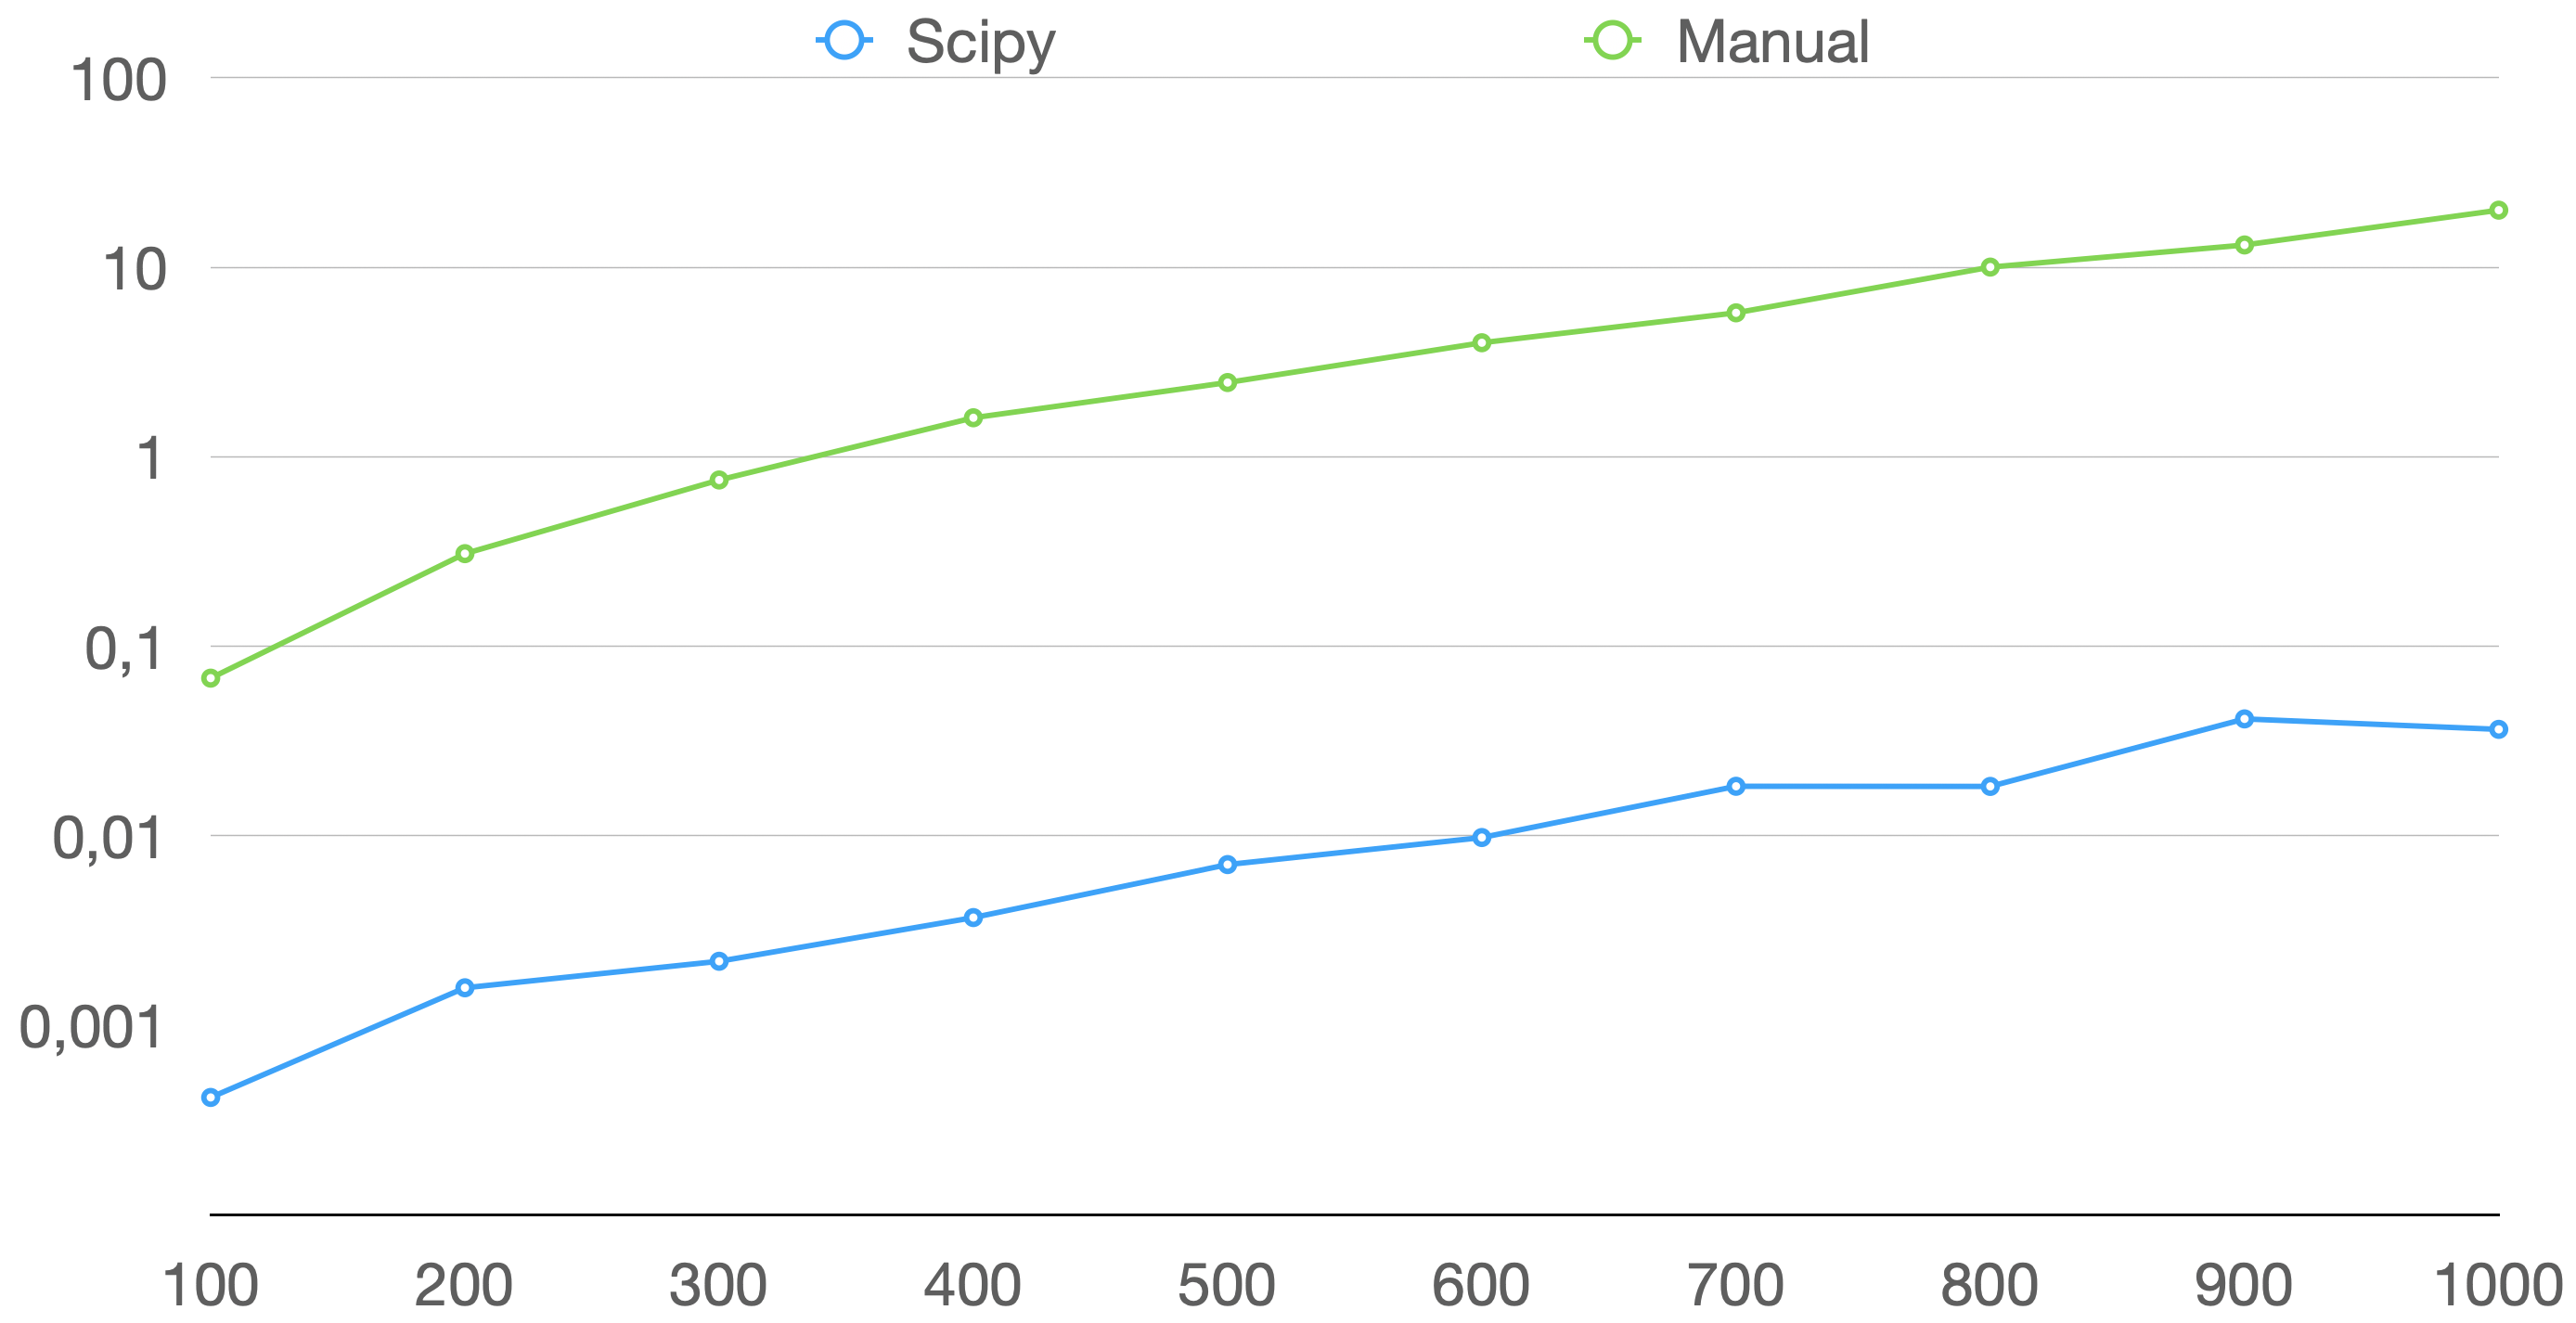
\includegraphics[width=\linewidth]{grafico}
\end{figure}

Nella figura sopra si possono notare come i tempi della DCT implementata a mano (Manual) siano nettamente superiori rispetto alla DCT implementata dal pacchetto di Python. Questo è del tutto normale in quanto le librerie sono sicuramente implementate meglio e più efficienti.

\newpage
Nella figura sotto sono riportati in una tabella tutti i tempi di esecuzione della DCT.

\begin{figure}[H]
	\centering
	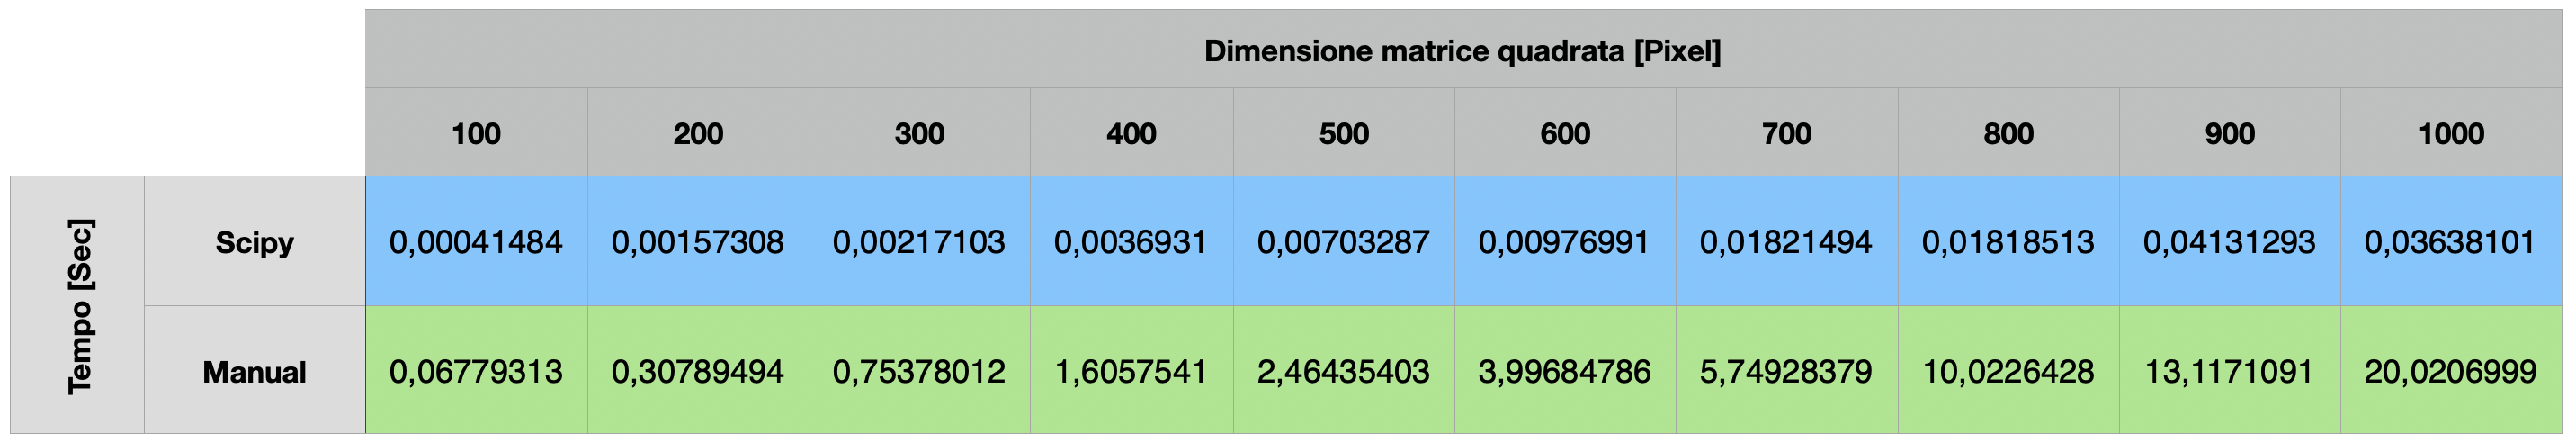
\includegraphics[width=\linewidth]{tabella}
\end{figure}

Si ricorda che i tempi di un algoritmo per DCT2 implementato da una libreria sono di circa $N^2 logN$, mentre i tempi di esecuzione di una DCT2 manuale si aggirano intorno a $N^3$, dove con $N$ si intende ovviamente la dimensione della matrice.

Detto ciò, i risultati finali dei tempi rispecchiamo a pieno tale regola, quindi possiamo tenerci soddisfatti circa la prima parte del progetto. 
\subsection{Parte 2}
Nella sezione corrente verranno presentati i risultati delle varie elaborazioni su grafici.

\end{document}